\chapter{Infraestructura}\label{cap.infraestructura}
En este capítulo se expondrán los principales componentes software utilizados, centrados, principalmente, en la conexión con la cámara y el desarrollo, entrenamiento y test de la red neuronal. Además, se expone una descripción de las bases de datos de las que se partirá para realizar las distintas pruebas sobre la red neuronal. Estas bases de datos serán luego modificadas y adaptadas para el problema concreto que se plantee, permitiendo obtener diversas conclusiones acerca del comportamiento de la propia red y, así, emplear la más adecuada. Por último, serán expuestas los parámetros empleados para evaluar el impacto del aprendizaje en las redes neuronales y que permitirán escoger la red más adecuada para el problema.\\

\section{Software}

\subsection{JdeRobot}\label{sec.jderobot}
JdeRobot~\footnote{http://jderobot.org} es una plataforma de software libre que facilita la tarea de los desarrolladores en el campo de la robótica, visión por computador y otras relacionadas, siendo este su principal fin.\\ 

Está escrito en su mayoría en el lenguaje C ++ y proporciona un entorno de programación basado en componentes distribuidas, de tal manera que una aplicación está formada por una colección de varios componentes asincrónos y concurrentes. Esta estructura permite la ejecución de los distintos componentes en diferentes equipos, estableciendo una conexión entre ellos mediante el middleware de comunicaciones ICE. Además, se obtiene gran flexibiidad a la hora de desarrollar las aplicaciones, ya que estos componentes pueden escribirse en C ++, Python, Java, etc. y todos ellos interactúan a través de interfaces ICE explícitas.\\ 

A pesar de que esta plataforma incluye una gran variedad de herramientas y librerías para la programación de robots, y de una amplia gama de componentes previamente desarrollados para realizar tareas comunes en este ámbito, su uso no es la verdadera finalidad del proyecto, ya que únicamente se centrará en la utilización de uno de sus componentes para facilitar la obtención de las imágenes.
\vspace{10pt}
\begin{description}
\item[Camera Server] \hfill 
\vspace{10pt}
\\
Se trata de un componente que permite servir a un número determinado de cámaras, ya sean reales o simuladas, a partir de un archivo de vídeo. Internamente utiliza \textit{gstreamer} para el manejo y el procesamiento de las diferentes fuentes de vídeo.\\
\vspace{-10pt}
\\
Para su uso, es necesario editar su fichero de configuración, adaptándolo a las necesidades concretas que plantee la máquina. Dentro de este fichero se permite especificar los siguientes campos:\\
\vspace{-20pt}
\begin{itemize}
    \item Configuración de la red, donde se indica la dirección del servidor que va a recibir la petición.
    \item Número de cámaras que se servirán.
    \item Configuración de las cámaras. Se podrán modificar los siguientes campos para cada cámara:
    \begin{itemize}
         \item Nombre y breve descripción
         \item URI: string que define la fuente de vídeo
     	 \item Numerador y denominador del frame rate
         \item Altura y anchura de la imagen
         \item Formato de la imagen
         \item Invertir o no la imagen 
    \end{itemize}
\end{itemize}
\end{description}

\subsection{Caffe}\label{sec.caffe}
Caffe~\cite{jia2014caffe} es una plataforma de aprendizaje profundo que permite el desarrollo, entrenamiento y evaluación de redes neuronales. Incluye, además, modelos y ejemplos previamente trabajados para un mejor entendimiento de las redes neuronales. Es una plataforma de software libre, escrito en C ++, que utiliza la librería CUDA para el aprendizaje profundo y permite interfaces escritas en Python o Matlab.\\ 

Esta plataforma es interesante por múltiples factores. Además de incluir diferentes ejemplos y modelos ya entrenados, lo que ofrece mayor agilidad a la hora de empezar a entender el funcionamiento de las redes neuronales, es destacable la velocidad que ésta ofrece para el entrenamiento de las redes y su posterior evaluación, ya que está prevista con varios indicadores que permiten evaluar la propia red y compararla con otras.\\ 

Su base se encuentra en las redes neuronales convolucionales explicadas en el Capítulo \ref{cap.introduccion}, utilizando un entrenamiento por lotes. En concreto, su estructura y funcionamiento básico queda explicado en la Figura~\ref{fig.redCaffe}.\\

\begin{figure}[H]
	\begin{center}
		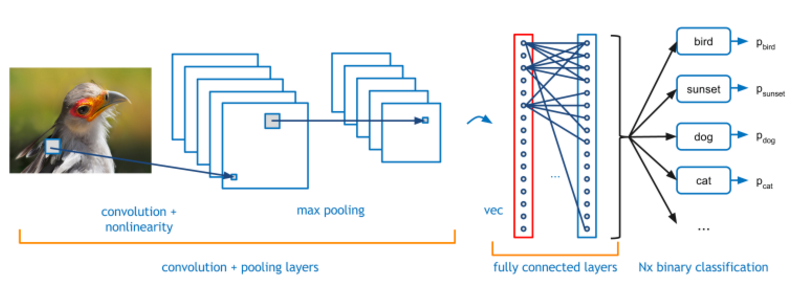
\includegraphics[width=0.6\textwidth]{figures/red_caffe}
		\caption{Estructura y funcionamiento básico de red en Caffe. Figura obtenida de~\cite{caffe}}
		\label{fig.redCaffe}
	\end{center}
\end{figure}

La plataforma utiliza una serie de capas (\textit{layers}), que, según su configuración y la distinta conexión entre ellas, permite la creación de diferentes redes neuronales. Estas capas se dividen en varios grupos, en función del tipo de entrada, el tipo de salida o la función que realiza cada una de ellas. Este trabajo no utiliza todas las capas existentes en la plataforma, a continuación se explicarán cada una de las capas empleadas, clasificadas según al grupo que pertenecen.
\vspace{20pt}
\begin{description}
\item[\textit{Data Layers}] \hfill 
\vspace{10pt}
\\
	Su uso se centra en la introducción de datos a la red neuronal, y estarán situadas siempre en la parte inferior de la misma. Estos datos provienen de diferentes vías que pueden ser: bases de datos eficientes como LMDB, utilizada en este trabajo, diréctamente desde la memoria o desde archivos en disco en HDF5 o formatos de imagen comunes.\\
	\vspace{-10pt}
	\\
	Dentro de esta capa es posible, además de especificar la ruta de los datos y el tamaño del lote (\textit{batch}), indicar la fase en la que se utilizarán los datos, entrenamiento o evaluación, así como algunos parámetros de transformación para el preprocesamiento de la imagen. En concreto, en este trabajo, se utilizarán datos de entrada para ambas fases y un factor de escala para establecer el rango de las imágenes en [0,1].
	\vspace{15pt}
	
\item[\textit{Vision Layers}] \hfill 
\vspace{10pt}
\\
	Este tipo de capas, típicamente toman una imagen de entrada y producen otra de salida, de forma que, aplicando una operación particular a alguna región de la entrada, se obtiene la región correspondiente de la salida. Caffe dispone de varias capas de este estilo, a continuación se comentan las dos utilizadas en el trabajo.
	\vspace{10pt}
	\begin{description}
	\item[\textit{Convolution Layer}] \hfill 
	\vspace{5pt}
	\\
		Realiza la convolución de la imagen de entrada con un conjunto de filtros de aprendizaje, cada uno produciendo un mapa de características en la imagen de salida. Se deben especificar datos como el número de salidas, el tamaño del filtro, el desplazamiento entre cada paso del filtro, y la inicialización y relleno de los pesos y \textit{bias}.
		\vspace{10pt}
	\item[\textit{Pooling Layer}] \hfill 
	\vspace{5pt}
	\\
		Combina la imagen de entrada aplicando una operación dentro de las regiones definidas por el filtro, siendo su finalidad la reducción del muestreo. Se especifican parámetros como el tipo de pooling a realizar, máximo, promedio o estocástico, el tamaño del filtro o el desplazamiento entre cada paso del filtro.
	\end{description}

\item[\textit{Common Layers}] \hfill
	\begin{description}
	\item[\textit{Inner Product}] \hfill 
	\vspace{5pt}
	\\
	Calcula un producto escalar con un conjunto de pesos aprendidos, y, de manera opcional, añade sesgos. Trata la entrada como un simple vector y produce una salida en forma de otro, estableciendo la altura y el ancho de cada \textit{bolb} en 1. Se establece el número de salidas, y la inicialización y relleno de los pesos y \textit{bias}.
	\vspace{10pt}
	\item[\textit{Dropout}] \hfill 
	\vspace{5pt}
	\\
	Durante el entrenamiento, únicamente, establece una porción aleatoria del conjunto de entrada a 0, ajustando el resto de la magnitud del vector en consecuencia, evistando así el sobre ajuste. Se debe indicar el ratio en un valor del 0 a 1, que indicará el porcentaje de muestras que se ignorarán.
	\end{description}

\vspace{15pt}	
\item[\textit{Activation / Neuron Layers}] \hfill  
\vspace{10pt}
\\
	En general estas capas son operadores de elementos que toman un \textit{bolb} inferior y producen uno superior del mismo tamaño. Existen varias capas con este funcionamiento en la plataforma, en concreto se empleará la \textit{\acrfull{relu}}.
	\vspace{10pt}
	\begin{description}
	\item[\textit{\acrshort{relu}}] \hfill  
	\vspace{5pt}
	\\
		Utiliza la función $y=max(0,x)$, cuya gráfica se define en la Figura~\ref{fig.reLu}, donde \textit{x} es la entrada a la neurona.
		\begin{figure}[H]
			\begin{center}
				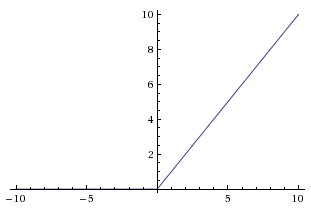
\includegraphics[width=0.5\textwidth]{figures/relu.jpeg}
				\caption{Función de activación \textit{{relu}}.}
				\label{fig.reLu}
			\end{center}
		\end{figure} 
	\end{description}
	
\item[\textit{Loss Layers}] \hfill 
\vspace{10pt}
\\
	El cálculo de la pérdida permite el aprendizaje mediante la comparación de la salida con un objetivo y la asignación de un coste para minimizarla. Se calcula mediante el paso hacia adelante. Existen diferentes medidas de las que se destacan dos.
	\vspace{10pt}
	\begin{description}
	\item[\textit{Softmax with Loss}] \hfill 
	\vspace{5pt}
	\\
		La función \textit{softmax} se utiliza a menudo en la capa final de un clasificador basado en redes neuronales. Se trata de una función que modifica un vector K-dimensional de valores reales arbitrarios a un vector K-dimensional de valores reales en el rango (0, 1] que suman 1.\\
		\vspace{-10pt}
		\\
		Esta capa es conceptualmente idéntica a una capa de \textit{softmax}, la cual calcula la función con el mismo nombre, seguida por una capa de pérdida logística multinomial, proporcionando un gradiente numéricamente más estable.
		Se calcula l pérdida como: 
		$$E = \frac{-1}{N} \sum\limits_{n=1}^N \log(\hat{p}_{n,l_n})$$
		Siendo $N$ el número total de muestras, $\hat{p}$ las probabilidades de cada etiqueta para cada muestra y $l_n$ las etiquetas existentes. Se definen las etiquetas existentes como $l_n\in[0, 1, 2, ..., K-1]$, siendo $K$ el total de clases. Adicionalmente, se debe multiplicar todo por $-1$ ya que se aplica el logaritmo a una probabilidad, oscilante entre 0 y 1, obteniendo un resultado negativo, y el que se desea obtener debe ser positivo.
		\vspace{10pt}
	\item[Accuracy] \hfill 
	\vspace{5pt}
	\\
		Esta capa calcula únicamente la tasa de acierto de la red, es decir, el número de aciertos en la clasificación referenciado al número total de muestras analizadas.
		Se calcula como:
		$$\frac{1}{N} \sum\limits_{n=1}^N \delta\{ \hat{l}_n = l_n \}$$

		Donde $\hat{l_n}$ es la etiqueta que la red decide en la clasificación y, al igual que en el caso anterior, $N$  es el número total de muestras y $l_n$ las etiquetas existentes. Por último, la función $\delta\{x\}$ se define como:
		$$\delta\{ \textup{condición}\} = \left\{ \begin{array}{lr} 1 &  \textup{si condición} \\ 0 & \mbox{resto} \end{array} \right.$$
	\end{description}
	
\end{description}
\vspace{10pt}

Por último, además de las capas y parámetros definidos anteriormente, Caffe, permite el desarrollo de un solucionador (\textit{solver}) en el que se podrán ajustar parámetros como el número de iteraciones totales que se ejecutarán, el de evaluación que se van a realizar, cada cuantas iteraciones se realizará esa evaluación, o se sacarán redes intermedias.\\

Para Caffe, el número de iteraciones no se corresponde con el número de veces que la red recorre la base de datos al completo, sino como las veces que se pasa por cada lote al completo. Esto viene dado porque, debido a la amplia dimensión de las bases de datos necesarias para desarrollar el aprendzaje profundo, según se explicación en el Capítulo~\ref{cap.introduccion}, será necesaria una división de la misma en pequeños lotes para que ordenador no se bloquee en el tratamiento de las mismas. De esta manera, se define el número de épocas, es decir, el número de veces que se recorre de manera completa la base de datos, con la siguiente expresión:\\
$$\textup{N.Epocas}=\frac{\textup{Tamaño lote de entrenamiento}\times \textup{Total iteraciones}}{\textup{Muestras entrenamiento}} $$\\

\subsection{DroidCam}\label{sec.droid}
DroidCam~\footnote{https://www.dev47apps.com/} es una aplicación que permite convertir un dispositivo móvil en una cámara web, estableciendo una conexión mediante WiFi/LAN, modo servidor wifi, o USB. Esta aplicación es muy usada para establecer videoconferencias a través de plataformas como Skype o Google+, entre otras aplicaciones. En este trabajo será usada para obtener el flujo de vídeo desde un dispositivo distinto a la webcam del ordenador, haciendo más sencillo el manejo del mismo.\\

La aplicación funciona con un componente cliente en el ordenador que instala los controladores de la cámara web y conecta el equipo con el dispositivo Android, que deberá tener instalada la misma aplicación.\\

Entre sus características principales destacan:
	\begin{itemize}
		\item Incluye sonido e imagen
		\item Conexión por diferentes medios
		\item Uso de otras apliaciones con DroidCam en segundo plano
		\item Cámara IP de vigilancia con acceso MJPEG
	\end{itemize}

\vspace{10pt}
\section{Bases de datos}

\subsection{MNIST}\label{sec.minst}
La base de datos \textit{\acrfull{mnist}}~\footnote{http://yann.lecun.com/exdb/mnist/} está formada por diferentes imágenes con números escritos a mano y consta de un conjunto de entrenamiento de 60.000 ejemplos y otro de prueba de 10.000 ejemplos. Es una buena base de datos para personas que quieren probar técnicas de aprendizaje y métodos de reconocimiento de patrones en datos del mundo real, mientras que dedican un mínimo esfuerzo a preprocesar y formatear. \\

Se trata de un subconjunto de una más grande, \textit{\acrfull{nist}}, en la que las imágenes originales en blanco y negro fueron normalizadas en el tamaño para encajar en un cuadro de 20x20 píxeles, preservando su relación de aspecto. Las imágenes obtenidas contienen niveles de gris como resultado de la técnica anti-aliasing utilizada por el algoritmo de normalización. Estas imágenes se centraron en una de 28x28 calculando el centro de masa de los píxeles y trasladando la imagen para situar este punto en el centro del campo 28x28.\\

Fue construida a partir de la Base de Datos Especial 3 y la Base de Datos Especial 1 del \acrshort{nist}, que contienen imágenes binarias de dígitos manuscritos.\acrshort{nist} originalmente designó SD-3 como su conjunto de entrenamiento y SD-1 como su conjunto de pruebas. Sin embargo, SD-3 es mucho más limpio y más fácil de reconocer que SD-1.Esto es debido a que SD-3 fue recogido entre los empleados de la Oficina del Censo, mientras que el SD-1 fue recogido entre los estudiantes de secundaria. Dado que para una buena extracción de conclusiones es necesario que el resultado sea independiente de la elección del conjunto de entrenamiento y de prueba entre el conjunto completo de muestras, fue necesaria la elaboración de un nuevo conjunto en el que ambas bases de datos estuviesen representadas de manera equitativa. Además, se aseguraron de que los conjuntos de escritores en el de entrenamiento y el de prueba son disjuntos.\\

\subsection{COCO}
Microsoft \textit{\acrfull{coco}}~\footnote{http://mscoco.org/} es un gran conjunto de datos de imágenes diseñado para la detección de objetos, segmentación y generación de subtítulos~\cite{veit2016cocotext}. Alguna de las características principales de este conjunto de datos son:
	\begin{itemize}
         \item Múltiples objetos en cada imagen
     	 \item Más de 300.000 imágenes
         \item Más de 2 millones de instancias
         \item 80 categorías de objetos
    \end{itemize}
    
Esta plataforma se ha desarrollado para varios retos, en concreto es de interés el reto de la detección, establecido en 2016. Se utilizan conjuntos de entrenamiento, prueba y validación con sus correspondientes anotaciones. \acrshort{coco} tiene tres tipos de anotaciones: instancias de objeto, puntos clave de objeto y leyendas de imagen, que se almacenan utilizando el formato de archivo \textit{\acrfull{json}} y comparten estructura de datos establecida en la Figura~\ref{fig.basicStruc}. \\

\begin{figure}[H]
	\begin{center}
		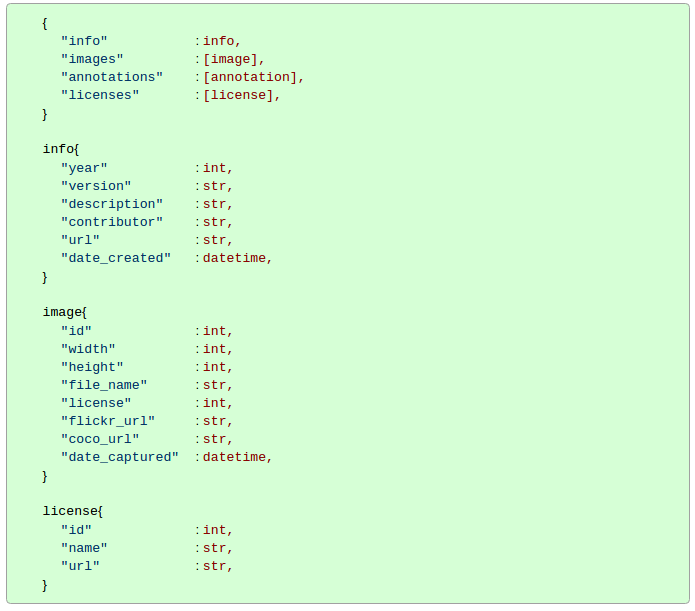
\includegraphics[width=0.8\textwidth]{figures/basic_structure_annotations.png}
		\caption{Estructura básica de anotaciones en \acrshort{coco}.}
		\label{fig.basicStruc}
	\end{center}
\end{figure} 

Para la detección son de interés las anotaciones de instancias de objetos, cuya estructura se muestra en la Figura~\ref{fig.objInst}.Cada anotación de instancia contiene una serie de campos, incluyendo el ID de categoría y la máscara de segmentación del objeto. El formato de segmentación depende de si la instancia representa un único objeto (\textit{iscrowd}~=~0), en cuyo caso se utilizan polígonos, o una colección de objetos (\textit{iscrowd}~=~1), en cuyo caso se utiliza \textit{\acrfull{rle}}. Debe tenerse en cuenta que un único objeto puede requerir múltiples polígonos, y que las anotaciones de la multitud se utilizan para etiquetar grandes grupos de objetos. Además, se proporciona una caja delimitadora para cada objeto, cuyas coordenadas se miden desde la esquina superior izquierda de la imagen y están indexadas en 0. Finalmente, el campo de categorías  almacena el mapeo del ID de categoría a los nombres de categoría y supercategoría.

\begin{figure}[H]
	\begin{center}
		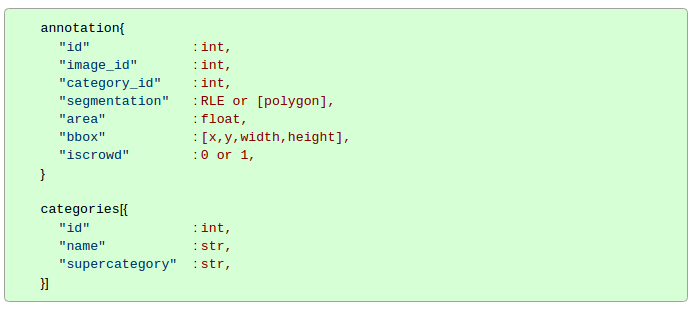
\includegraphics[width=0.8\textwidth]{figures/instancia_objetos.png}
		\caption{Estructura de instancias de objetos en \acrshort{coco}.}
		\label{fig.objInst}
	\end{center}
\end{figure}

\subsection{VOC}
El objetivo del desafío de \textit{\acrfull{voc}} \cite{Everingham10} es investigar el desempeño de los métodos de reconocimiento en un amplio espectro de imágenes naturales. Para ello, se requiere que los conjuntos de datos \acrshort{voc} contengan variabilidad significativa en términos de tamaño del objeto, orientación, pose, iluminación, posición y oclusión. También es importante que los conjuntos de datos no muestren sesgos sistemáticos, por ejemplo, favoreciendo imágenes con objetos centrados o una buena iluminación. Del mismo modo, para garantizar un entrenamiento y una evaluación precisa, es necesario que las anotaciones de imagen sean consistentes, precisas y exhaustivas para las clases especificadas.\\

Teniendo claros estos conceptos, en 2007, se llevó a cabo una recolección de imágenes, como las mostradas en la Figura~\ref{fig.voc_example}, formando el conjunto de datos \textit{\acrshort{voc}}\textit{2007}~\cite{pascal-voc-2007}. Este conjunto dispone de dos grandes bases de datos, una de ellas compuesta por un conjunto de validación y otro de entrenamiento, y la otra con un único conjunto de test. Ambas bases de datos contienen alrededor de 5000 imágenes en las que se representan, apróximadamente, 12.000 objetos diferentes, por lo que, en total, este conjunto dispone de unas 10000 imágenes en las que se reperesentan unos 24000 objetos. En el año 2012 se modifica este conjunto, aumentando a 11530 el número de imágenes con representación de 27450 objetos diferentes~\cite{pascal-voc-2012}.

\begin{figure}[H]
	\begin{center}
		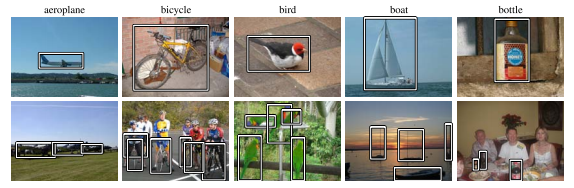
\includegraphics[width=0.7\textwidth]{figures/vocexample}
		\caption{Ejemplos de imágenes en \acrshort{voc}. Imagen tomada de~\cite{Everingham10}}.
		\label{fig.voc_example}
	\end{center}
\end{figure}

Dado que la finalidad de este conjunto de datos es permitir el desarrollo tanto de la clasificación de objetos como la detección de los mismos, será necesario que estas imágenes contengan una serie de anotaciones. Entre otras cosas, estas anotaciones contienen dos atributos importantes para ambas tareas:

\begin{itemize}
	\item Para la \textbf{clasificación}, se debe indicar la clase de objeto que es. Los objetos de este conjunto estan clasificados en 20 clases diferentes. En la Figura~\ref{fig.clasesVOC} se puede observar la división que se hace de cada una de las clases y las distintas clases existentes.
	\item Para la \textbf{detección}, será necesario indicar, para cada objeto, la \textit{bounding box}. Se trata de un cuadro delimitador alineado con el eje que rodea la extensión del objeto visible en la imagen, permitiendo identificar el objeto en la imagen.
\end{itemize}
\begin{figure}[H]
	\begin{center}
		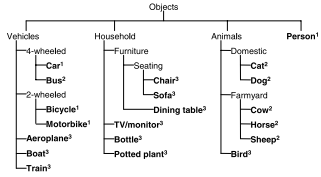
\includegraphics[width=0.7\textwidth]{figures/vocclasses}
		\caption{Estructura de las clases en \acrfull{voc}2007. Imagen tomada de~\cite{Everingham10}}. El año de inclusión de cada clase en el desafío está indicado por
		superíndices: $2005^1$, $2006^2$, $2007^3$.
		\label{fig.clasesVOC}
	\end{center}
\end{figure}

\section{Evaluación de prestaciones} \label{sec.prestaciones}
Existen multitud de parámetros que permiten la evaluación de las redes neuronales, sin embargo, en este proyecto, todas las comparaciones se centrarán en cinco de ellas: \textit{accuracy}, \textit{loss}, matriz de confusión, \textit{precision} y \textit{recall}~\cite{pullum2007guidance}.\\

Las dos primeras fueron explicadas en la Sección~\ref{sec.caffe}, por lo que no se ahondará más sobre ellas. Las tres restantes serán explicdas más profundamente, y de manera totalmente teórica a continuación.

\subsection{Matriz de confusión}
Una matriz de confusión (Kohavi y Provost, 1998) contiene información sobre las clasificaciones reales y predichas hechas por un sistema de clasificación. El rendimiento de estos sistemas se evalúa comúnmente utilizando los datos de la matriz~\cite{metrics}. En la Figura~\ref{fig.matriz} se muestra un ejemplo sencillo de la construcción de esta matriz donde:
\begin{itemize}
	\item \textbf{\textit{a}} es el número de predicciones correctas de que una instancia es negativa
	\item \textbf{\textit{b}} es el número de predicciones incorrectas de que una instancia es positiva
	\item \textbf{\textit{c}} es el número de predicciones incorrectas de una instancia negativa
	\item \textbf{\textit{d}} es el número de predicciones correctas de que una instancia es positiva.
\end{itemize}

\begin{figure}[H]
	\begin{center}
		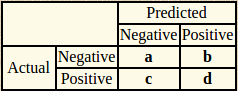
\includegraphics[width=0.3\textwidth]{figures/matrizexample}
		\caption{Ejemplo sencillo de matriz de confusión. Imagen tomada de~\cite{metrics}}.
		\label{fig.matriz}
	\end{center}
\end{figure}

Además de ayudar con el cálculo de \textit{precision} y \textit{recall}, es importante mirar la matriz de confusión para analizar sus resultados, ya que también proporciona información importante sobre dónde el clasificador funciona mal~\cite{metrics2}. Para que una matriz proporcione información sobre el correcto funcionamiento de un clasificador se obtendrán valores altos en la diagonal, y lo más pequeños posible en el resto de celdas de la misma.

\subsection{\textit{Precision}}
Se trata de la proporción de los casos positivos predichos que fueron correctos~\cite{metrics}. Para obtener este valor en el ejemplo sencillo anteriormente explicado se utiliza la fórmula:
$$P = \frac{d}{b+d} $$
Donde $P$ es el valor de \textit{precision} y $b$ y $d$ los mismo valores explicados en la sección anterior.\\

En un caso más complejo en el que la clasificación no sea binaria, se deben de tener en cuenta todas las clases, por ello la fórmula queda expresada de la siguiente forma~\cite{metrics2}:
$$P = \frac{TP_X}{TP_X + FP_X} $$
Donde:
\begin{itemize}
	\item $TP_X$ se corresponde el número de verdaderos positivos para la clase $X$, es decir, el valor de aciertos correspondiente para dicha clase, situado en la diagonal.
	\item $FP_X$ se corresponde el número de falsos positivos para la clase $X$, es decir, el número de veces que se predijo dicha clase sin haber sido producida, correspondiente con la suma del resto de celdas en la misma fila.
\end{itemize}

\subsection{\textit{Recall}}
Se trata de la proporción de casos positivos que fueron correctamente identificados~\cite{metrics}. Para el ejemplo sencillo se calcula mediante la siguiente expresión:
$$R = \frac{d}{c+d} $$
Donde $R$ es el valor de \textit{recall} y $c$ y $d$ los mismo valores explicados anteriormente.\\

Al igual que en el caso de la sección anterior, en caso de tener una clasificación multiclase se deberás tener en cuenta todas ellas, utilizando para ello la expresión~\cite{metrics2}:
$$R = \frac{TP_X}{TP_X +FN_X} $$
Donde $TP_X$ se corresponde con lo explicado en la sección anterior y $FN_X$ se corresponde con los falsos negativos para la clase $X$, es decir, el número de veces que se predijo errónamente otra clase habiéndose producido $X$, correspondiente con la suma del resto de la columna. 